Figure~\ref{fig:4:fw} in Chapter~\ref{chap:cc.fw} shows the structure of the
congestion control framework described in this thesis. The framework
categorizes \emph{In-path} and \emph{Out-of-path} sources and
\emph{out-of-band} signaling for implementing congestion control (corresponds
to \emph{Block B and D} of Figure~\ref{fig:4:fw}), which are discussed in this
chapter. This chapter is based on our work on network assisted congestion
control, which is documented in \citepub{c:3grc}, \citepub{c:glass} and
\cite{glass:patent}.

In a 3G network, mobility, cell loading, handovers and other factors can
affect the throughput available to each user and the varying network capacity
affects the video quality~\cite{diaz2007evaluating}. Deployments of GPRS, 3G
and LTE show that there are still geographical areas where capacity is
constrained~\cite{Curcio:glass, 6576402}. These constrained geographical areas
may occur due to fading and interference from large building structures or
closed or inaccessible areas (e.g., tunnels, boats on lakes or in the
archipelago, rural areas).

In \citepub{c:3grc}, when the available link capacity changes at a base
station, it notifies the endpoint connected to it about the current capacity.
Based on the notifications the sender adapts the media sending rate. Hence,
this paper covers the \emph{in-path} sources and \emph{out-of-band} signaling
of the framework defined in Chapter~\ref{chap:cc.fw}. We evaluate the
performance of employing network-assistance for congestion control in a
simulated environment using real-world 3G traces.

In \citepub{c:glass}, we explore the use of coverage maps for congestion
control. The map server collect throughput information from the mobile
clients, which also add geo-location information along with the throughput
information. This assists the map server to build a bandwidth and coverage map
and is queried by the mobile to predict coverage outage. This paper covers the
\emph{out-of-path} sources (e.g., coverage map) signaling congestion cues
\emph{out-of-band} to the endpoints. The paper also discusses the protocol and
implementation aspects of such a service. Lastly, we evaluate the performance
of using a coverage map for congestion control by collecting 3G traces and
emulating it in our testbed.

\section{In-path Congestion Cues}

% ECN, PCN, BW indication

In some network deployments, routers along the media path are capable of
detecting congestion before the queue overflows, typically, using active queue
management (e.g., RED). A router marks a packet, indicating that the packet
experienced congestion and the router would soon drop packets for this
flow~\cite{rfc3168}. The receiver on receiving this indication keeps a counter
for the number of ECN marked IP packets and signals it to the sender. For
performing congestion control, the sender typically treats the count of ECN
marked packets as lost packets~\cite{rfc6679}. For example, the sender uses
the sum of the reported loss events and the reported ECN events as the
\emph{p} (loss) value in the TFRC equation. Network-Assisted Dynamic
Adaptation (NADA)~\cite{rmcat-nada} propose a delay-based congestion control,
the receiver measures congestion by aggregating the packet loss count,
reported ECN markings, and one-way delay measurements into a single cue. The
sender calculates the new rate based on the variation in the delay cue
compared to earlier measurements and the priority of the multimedia
stream~\cite{pv-nada}.

\begin{figure}
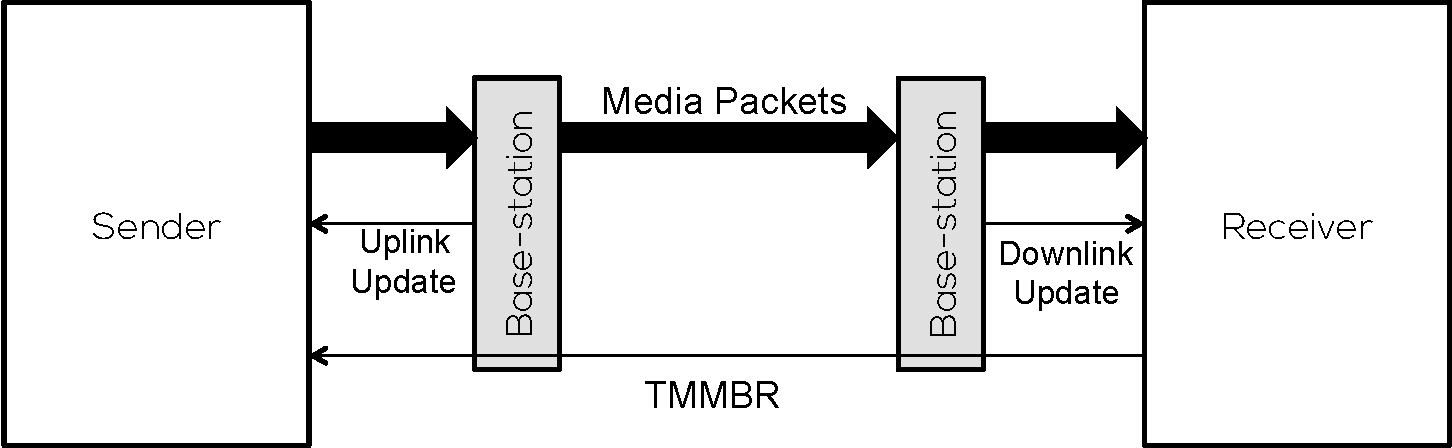
\includegraphics[width=\textwidth]{chap8-fig-tmmbr}
  \caption{Endpoints receiving capacity indication from the middleboxes
  (TMMBR) for implementing congestion control.}
\label{fig:cc:tmmbrab}
\end{figure}

In wireless networks, such as 3G/LTE, the last hop is typically the bottleneck
because the core network is well provisioned. In \citepub{c:3grc}, we
implement a network-assisted congestion control scheme, wherein, base-stations
(along the media path) notify the mobile terminals about the available link
capacity. In TMMBR-A, the base-stations notify both the sending and receiving
endpoints about the available capacity, i.e., the sender is notified about the
uplink capacity and the receiver is notified about the downlink capacity. If
an endpoint sends and receives data, it is notified asynchronously about the
uplink and downlink capacity. Figure~\ref{fig:cc:tmmbrab} shows a schematic
representation about the interaction between the middleboxes and the
endpoints. In TMMBR-B, the receiving endpoint is solely notified about the
downlink capacity. Both TMMBR-A and TMMBR-B employ a co-operative congestion
control scheme, wherein the receiver sends a TMMBR request to the sender
containing the current downlink capacity. In TMMBR-A the sender also receives
a notification about the uplink capacity from the base-station, hence,
comparing the request from the receiver and the notification from the
base-station, it chooses the minimum of the two values as the new sending
rate. In TMMBR-B, the sender implements calculates the \emph{sender's
estimate} (similar to the one described in~\ref{cc:co-op}) and chooses the
minimum of the sender's estimate and the receiver's bit rate request.
Figure~\ref{fig:tmmbn} shows the performance of TMMBR-A and TMMBR-B, where
both endpoints are sending media over a 3G network.

\begin{figure}
  \centerline{
    \subfloat[TMMBR-A]{
      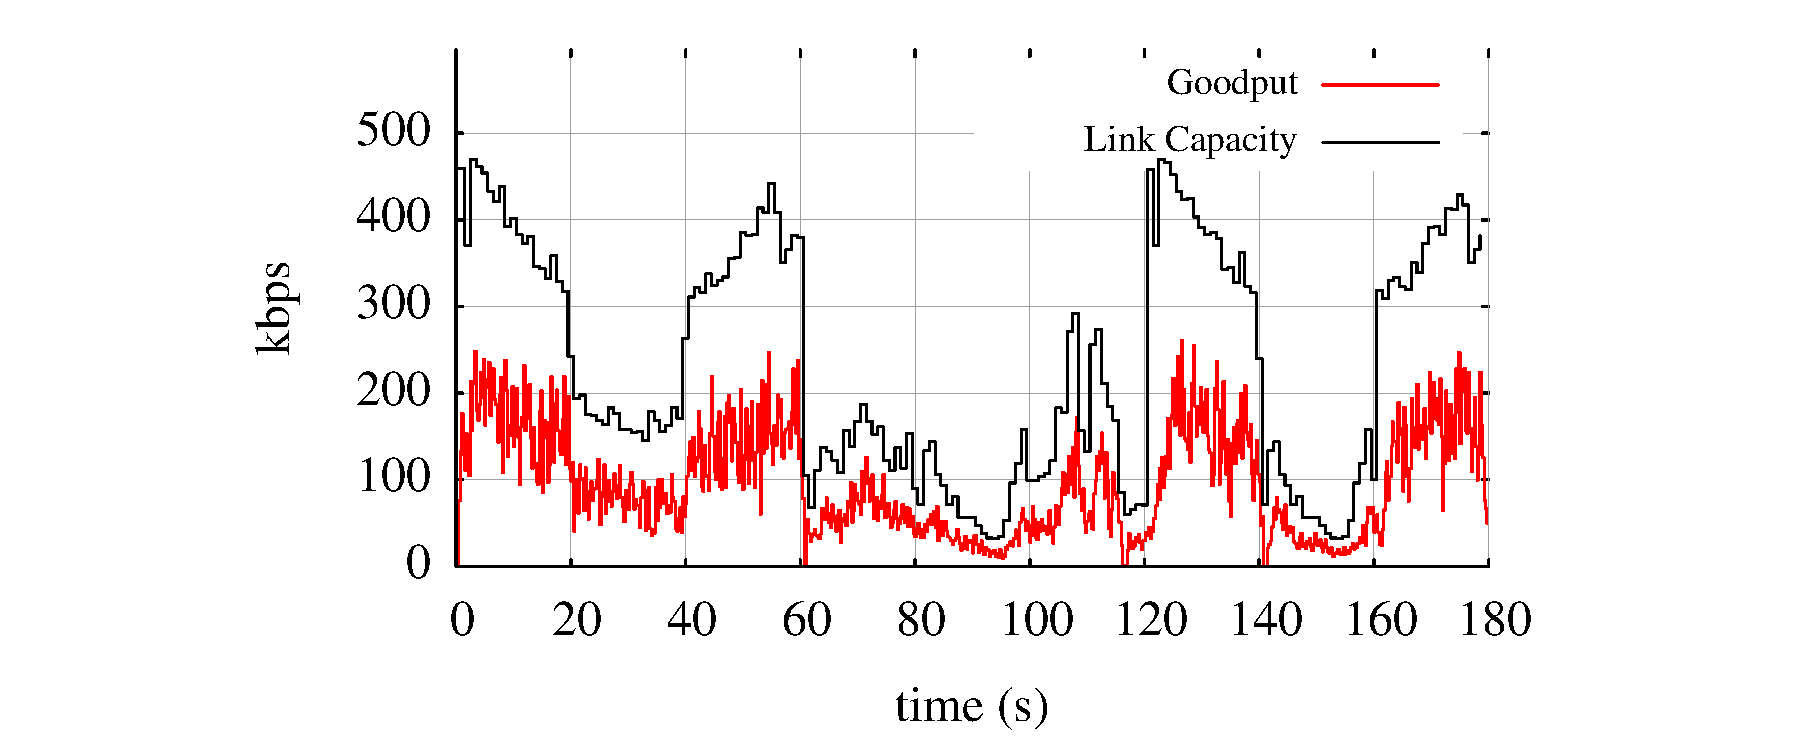
\includegraphics[width=0.5\textwidth, clip=true, trim=3cm 0 4.5cm 0]
      {chap8_graph_3g_tmmbr_a}
    }
    \subfloat[TMMBR-B]{
      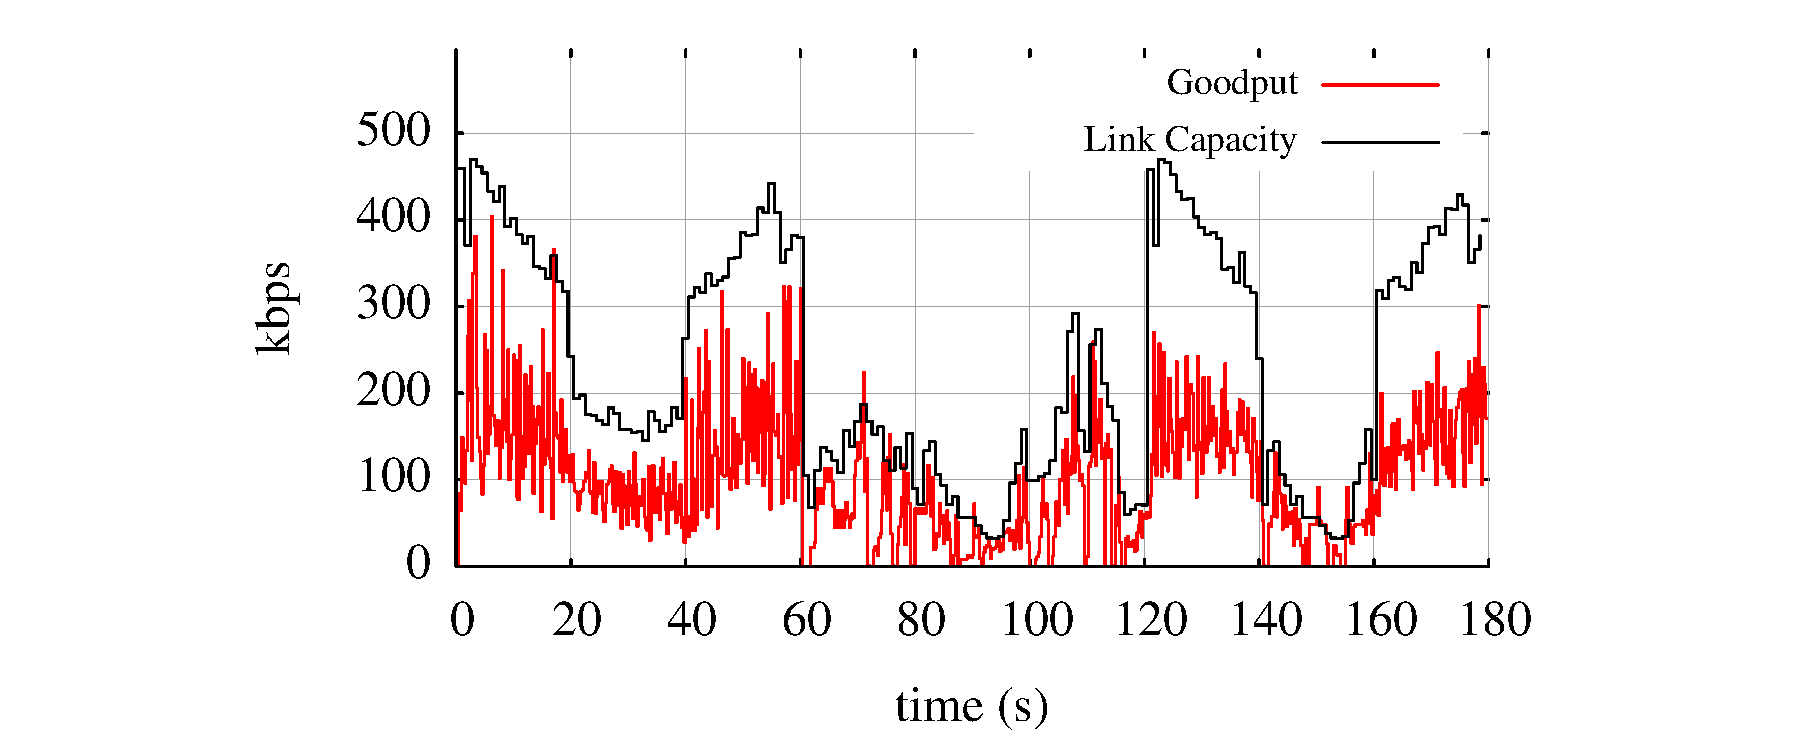
\includegraphics[width=0.5\textwidth, clip=true, trim=3cm 0 4.5cm 0]
      {chap8_graph_3g_tmmbr_b}
    }
  }
  \caption{The plots show the performance of bandwidth indications by the base
  stations a) TMMBR-A: both terminals are assisted, b) TMMBR-B: the receiver
  is only assisted.}
  \label{fig:tmmbn}
\end{figure}


\section{Out-of-path Congestion Cues}

% Congestion map

Service Maps are presented in~\cite{1630563} and the measurement based
approach is proposed in~\cite{Aravinda:2008p14}. GPS-based congestion control
is introduced in~\cite{Yao:2008p21}, and evaluated in different
scenarios~\cite{Yao:2009p57}, \cite{Yao:2010p64}, but they take signal
strength as an influential factor for rate-control and show that predicting
based on signal strength alone is insufficient. Yet, their results indicate
that past information can be used to predict future network characteristics.

To overcome these challenges, in \citepub{c:glass}, we implement a bandwidth
coverage map that collects connectivity information from the users
(\emph{crowd-sourcing}) and calculates the available capacity at the reported
geographical locations. \cite{6012045} also proposes a similar architecture
(\emph{bandwidth lookup service}) to the one in \citepub{c:glass} and uses
different types of averaging algorithms to predict future network
characteristics in Dynamic Adaptive Streaming over HTTP (DASH). While the
averaging algorithm is not a focus of this thesis, we use
K-means~\cite{Kanungo:2002:LSA:513400.513402} and K-nearest neighbor
(K-NN)~\cite{Iwerks:2003:CKN:1315451.1315496} algorithms to form regions with
similar bandwidth. Details of the averaging algorithms employed by our
coverage map server are discussed in~\cite{sharmistha-thesis}. Additionally,
\cite{Riiser:2012:2240136} proposes fetching the bandwidth along a travel
route in steps of 100 meters, which we find limiting. Instead we propose
multiple methods for discovering areas with poor connectivity and show that
not only looking up future bandwidth but also when to vary the sending rate
affects the usefulness of the service. A preliminary analysis using
simulations of our system is done in~\cite{Curcio:glass}.

\begin{figure}
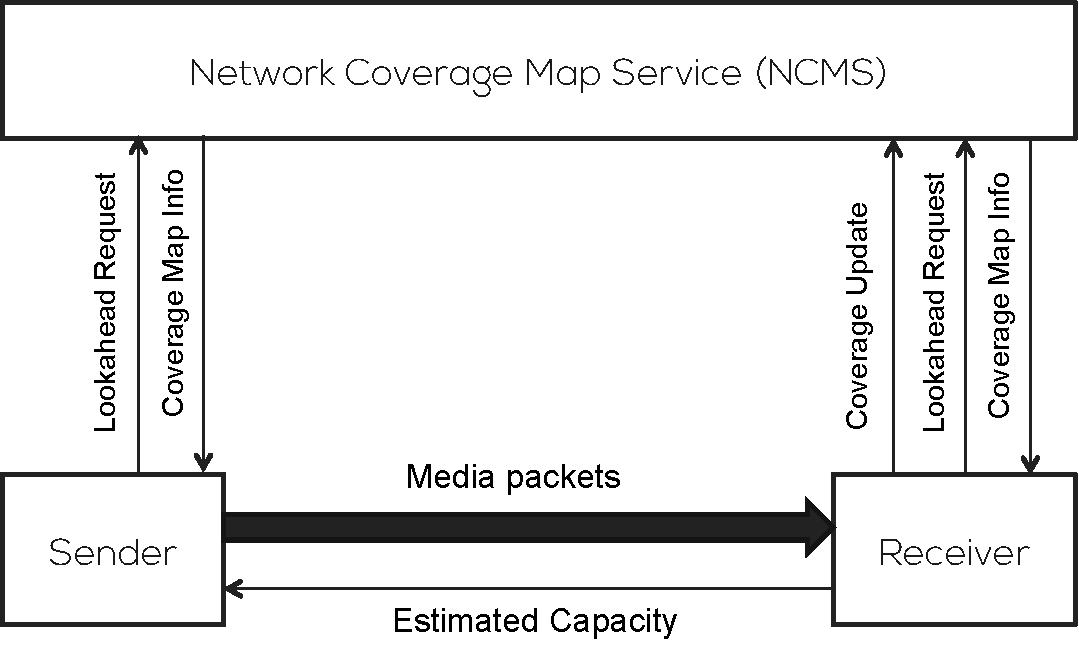
\includegraphics[width=\textwidth]{chap8-fig-ecv}
  \caption{Endpoints using a Network Coverage Map Service to send coverage
  updates, query for upcoming congestion and receive coverage updates.}
\label{fig:cc:ecv}
\end{figure}


In \citepub{c:glass}, we present a mechanism enabling an endpoint (usually a
receiver) to proactively react to upcoming capacity limitations in wireless
access networks. We enable this by implementing three steps,
Figure~\ref{fig:cc:ecv} shows the interaction between the endpoints and the
Network Coverage Map Server (NCMS). First, each endpoint receiving a media
stream monitors the throughput and its geolocation and reports it to the NCMS.
Figure~\ref{fig:glass:map} shows the throughput around the university area in
Espoo. Second, each endpoint is capable of querying the NCMS for upcoming
congestion (known as \emph{lookahead}). It can \emph{lookahead} using one of
the following methods: known travel rote, area lookahead or by subscribing to
areas with poor coverage\footnote{Areas where the expected channel capacity is
lower than the media bit rate}. Figure~\ref{fig:glass:map} shows a graphical
representation of the average throughput for a \emph{area lookahead} and a
\emph{known travel route}. Third, for each lookahead requests, the NCMS
responds with an coverage map info, i.e., the expected throughput at every
geolocation along the route or requested area.


\begin{figure}
  \centerline{
    \subfloat[Map Area Lookahead]{
      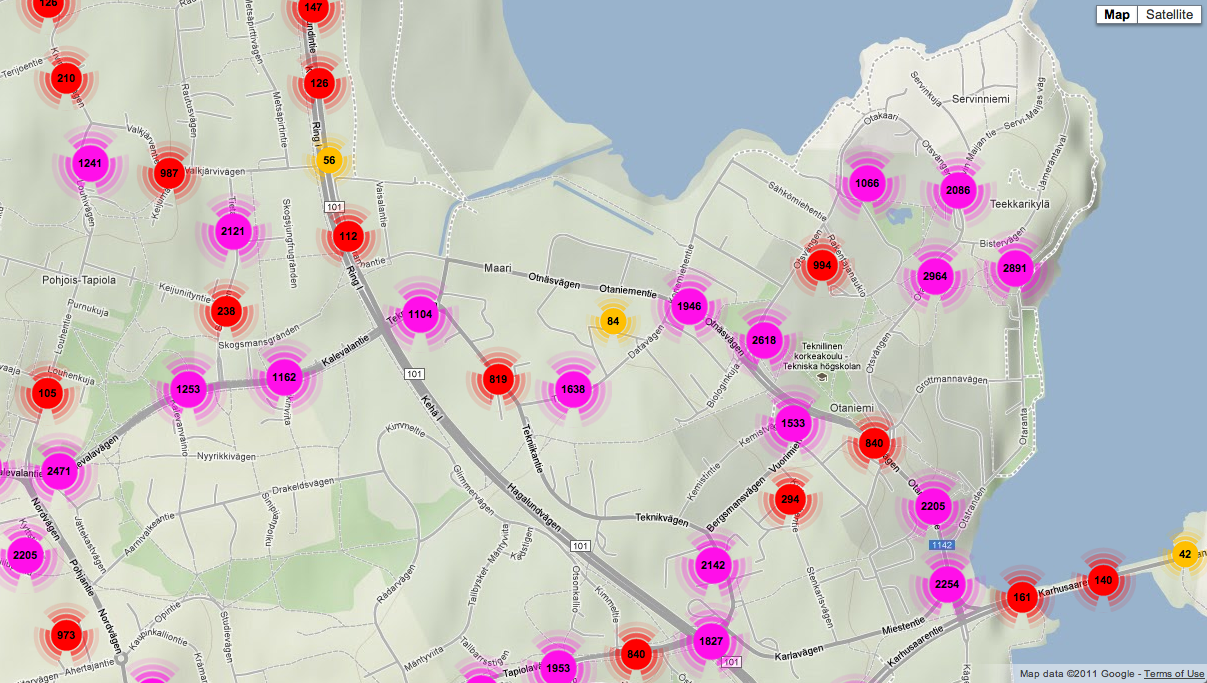
\includegraphics[width=0.8\textwidth]
      {chap8-fig-ota-tr-net-02}
    }
  }
  \centerline{
    \subfloat[Known Travel Route Lookahead]{
      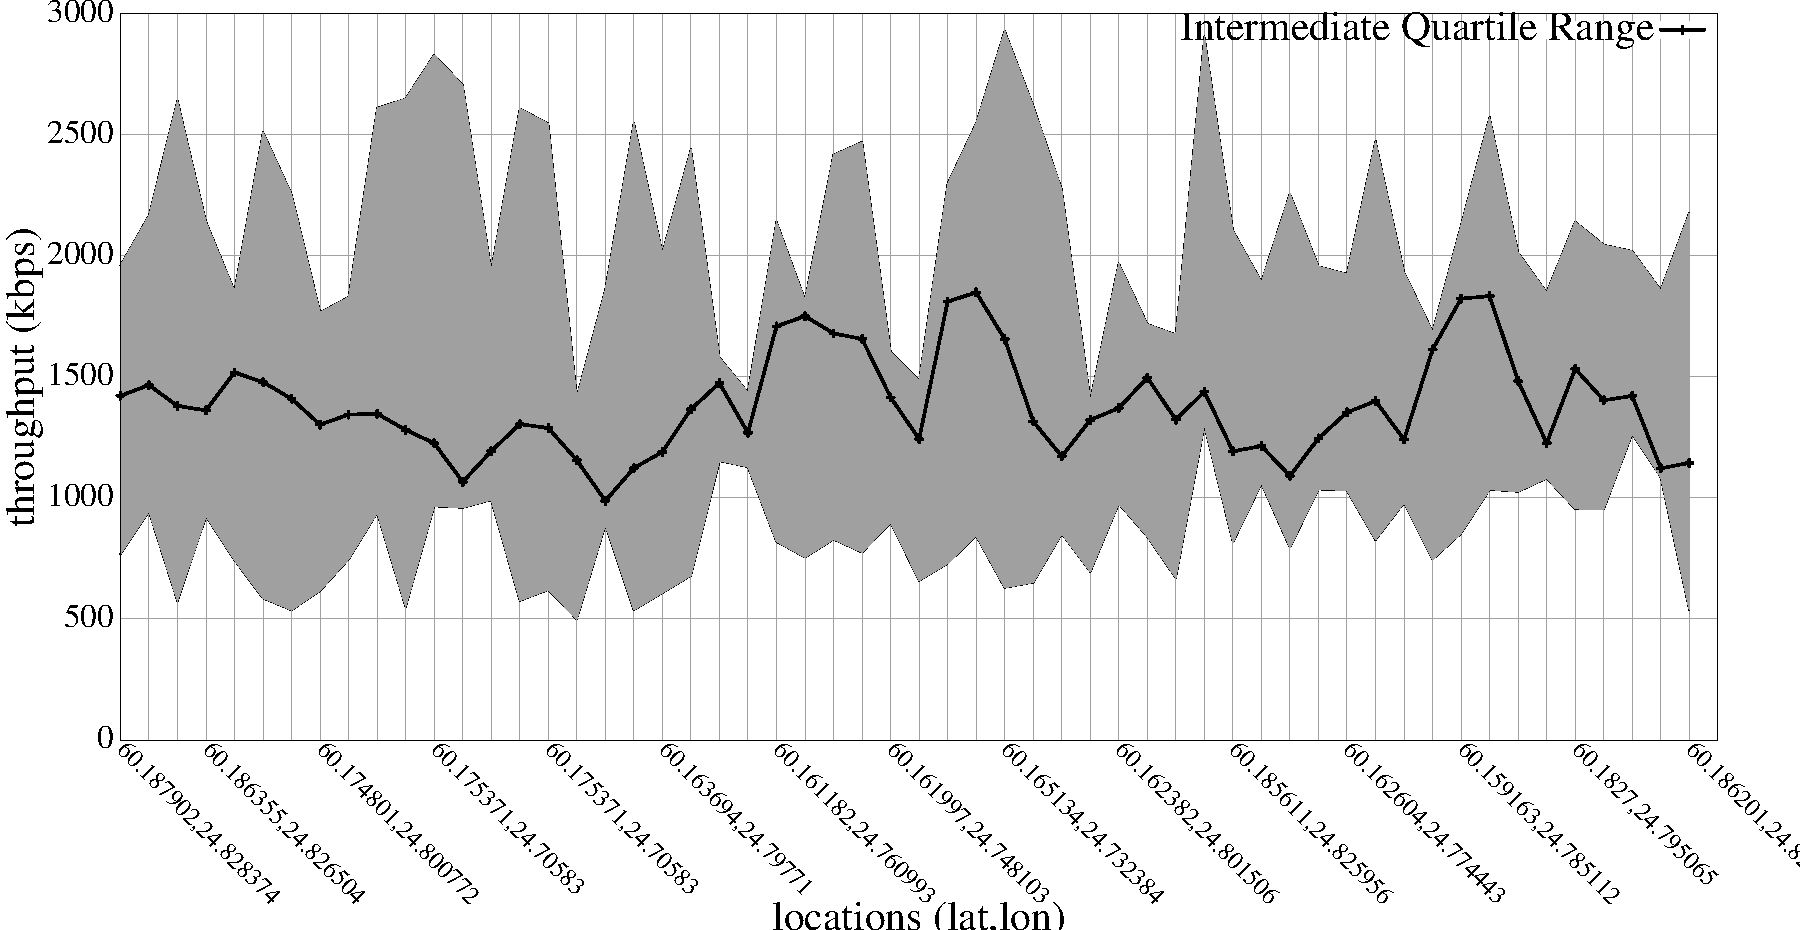
\includegraphics[width=0.8\textwidth]
      {chap8-graph_route_thin_throughput}
    }
  }
  \caption{a) A map of the available capacity around Otaniemi (university
  area). b) Example of the average and the Inter Quartile Range
  ($IQR=\pm1\sigma$) throughput along a known route. The data in both
  representations are captured over several days.}
  \label{fig:glass:map}
\end{figure}

The receiver uses these hints provided by the NCMS to implement congestion
control. It sends an \emph{estimated capacity vector} (a data structure
containing a time-series of available throughput, thus preserving user's
location privacy) are sent to the sender, which can alter the sending rate
based on the received information. The sender has the following techniques to
change the sending rate: 1) change the encoding rate, 2) perform rate-switch,
or, 3) pre-buffer. Changing the encoding rate is only possible in interactive
real-time media, because the RTP sender co-operates with the encoder to modify
the encoding rate. Rate-switching is only possible for stored content or live
content where a media stream is encoded at different bit rates and the
application switches between the stored media files, this performance of the
congestion control depends on the granularity of the chosen bit rates for the
media stream. Lastly, pre-buffering provides a more consistent experience to
the user, because the technique attempts to maintain the same media encoding
rate by modulating the sending rate. It is only applicable to stored content,
the application, typically, reads-ahead in the media stream and sends more
data whenever before it detects poor coverage.

In \citepub{c:glass}, we stream video from a server to mobile clients moving
around the city, mainly using public transport. The NCMS collected the
throughput traces, thereafter, we conduct simulated experiments of users
traveling at different vehicular speeds through the Helsinki region. In total,
the NCMS collected over 400,000 updates over a month of operation (about 40-50
bus-trips). For 6 geographical areas, the NCMS received more than 10,000
updates (\emph{Otaniemi}, Helsinki City Center) while on average each
geographical had around 100 updates.


\begin{table}
  \begin{center}
\begin{tabular}{ccccccc} \hline
Method & $SR_{avg}$ & $PSNR_{avg}$ & $\sigma_{PSNR}$ & PLR \\ \hline
% & $buffer_{max}$\\ \hline
No adaptation   & 865   & 27.48 & 4.55  & 6.6 \\
Omniscient      & 929   & 43.12 & 1.9   & 0.33 \\ 
Rate-switching  & 881   & 42.75 & 2.21  & 0.0  \\ 
Late scheduling & 1014  & 48.43 & 0.18 & 0.0  \\ \hline
\end{tabular}
\caption{A bus ride with good 3G coverage.}
\label{table-glass-sim7res}
\end{center}
\end{table}

Table~\ref{table-glass-sim7res} compares the results for the different schemes
and Figure~\ref{fig:glass:sim7res} shows the sending/receiver rate variation
to channel throughput for one out of 10 simulation runs. In this scenario the
user moves smoothly through the locations along the route and the receiver
performs \emph{lookahead} queries to fetch coverage information. In this
scenario, there are intermittent gaps in coverage but overall the throughput
at most locations is above the required media rate. The \emph{omniscient
algorithm}\footnote{The endpoint is aware of the exact end-to-end channel
capacity and performs the perfect rate-adaptation.} provides the best
rate-adaptation but since it is unable pre-buffer, the PSNR ($PSNR_{avg}$=43)
is lower than that of late scheduling ($PSNR_{avg}$=48). Alternatively,
performing \emph{no adaptation}\footnote{Endpoints perform no congestion
control and stream at a constant bit rate and periods when the link capacity
falls below the media rate, will cause losses} causes frequent pausing and
packet loss which is reflected in the low PSNR ($PSNR_{avg}$=27).

\begin{figure}
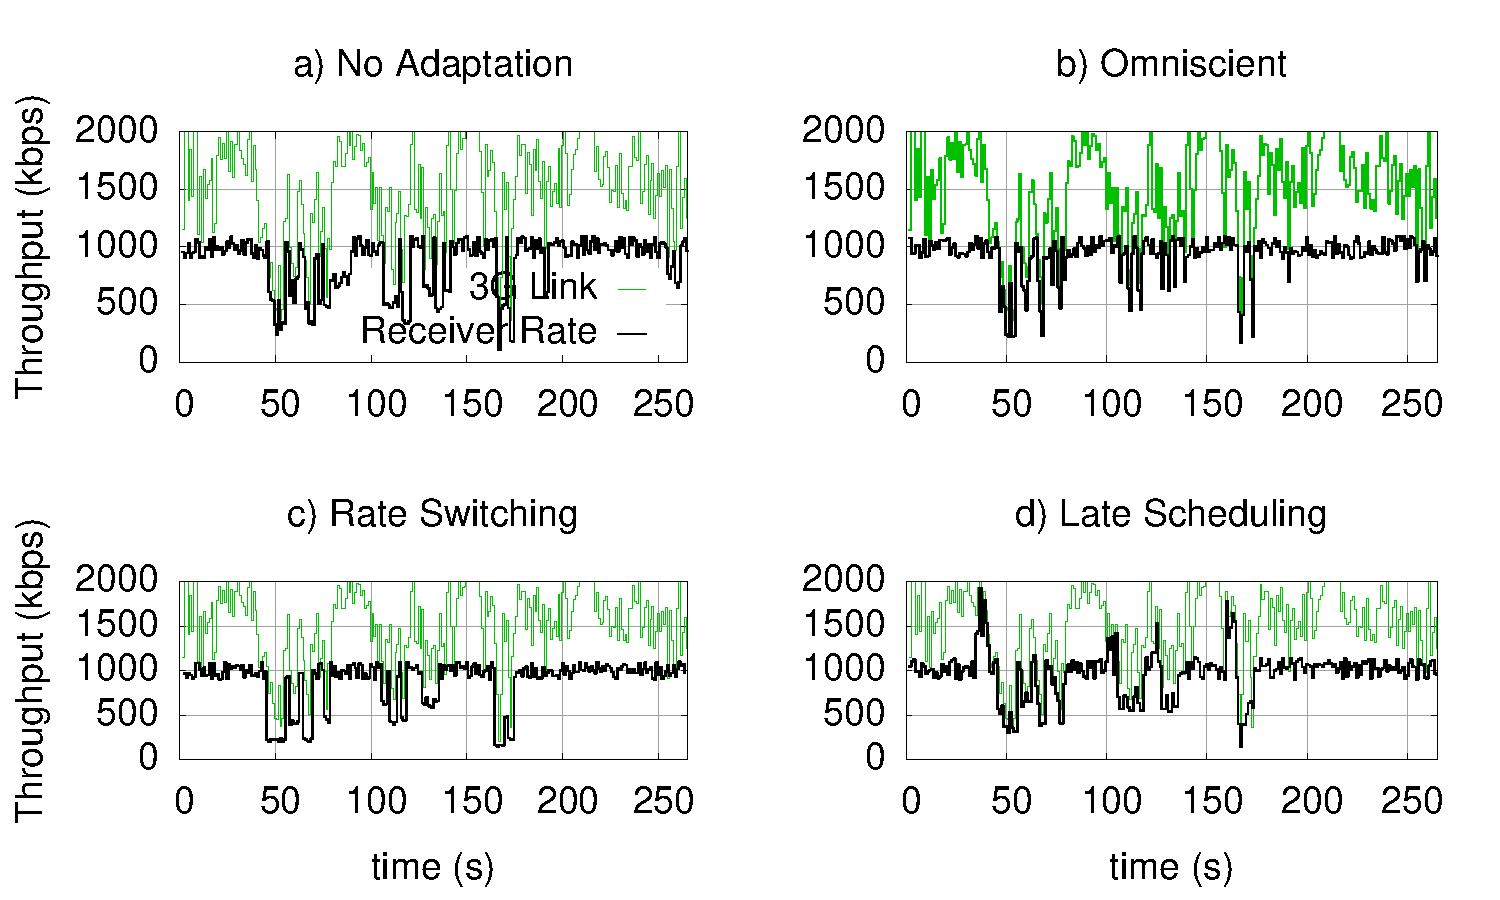
\includegraphics[width=\textwidth]{chap8-graph-sim7-3}
  \caption{The plot shows the variation of sending rate to 3G link capacity
  based on a) no adaptation b) Omniscient c) Rate-switching d) Late scheduling
  when there are few coverage holes and good connectivity between them.}
\label{fig:glass:sim7res}
\end{figure}

\emph{Rate-switching}\footnote{Endpoints perform short \emph{lookahead}
requests and is only able to detect outage moments before the user arrives at
the location with poor connectivity. In this case, the receiver sends a TMMBR
message (with lowest available bit rate in the area) before entering the area
and another one after the exiting the area (to reset the bit rate). The sender
reacts by switching the media stream to the closest available media rate.} has
comparable PSNR ($PSNR_{avg}$=42.75) to \emph{Omniscient} and has no packet
losses. \emph{Rate-switching} avoids all drops by switching to values lower
than the average or minimum reported throughput. \emph{Late
scheduling}\footnote{The receiving endpoint performs lookahead requests and
tries to detect areas with poor coverage much before the user arrives at those
locations. To reduce the impact of changing routes, the streaming client uses
the congestion control algorithm proposed in \citepub{c:glass}.} outperforms
the rest of the schemes in terms of PSNR ($PSNR_{avg}$=48.43) because it
predictively pre-buffers content and does not have to rate-switch. This is
largely due to the low density of coverage holes and good connectivity between
them. In the case of interactive multimedia communication implementing
network-assisted congestion cues, we expect the performance of the congestion
control to be at least that of rate-switching because the sender will be able
to reduce and increase the sending rate preemptively without probing.

We find that the information provided by the NCMS is suitable for both
predictive rate-switching and pre-buffering and helped in avoiding almost all
packet losses in the scenarios we investigated, noticeably increasing video
quality. This system can be adapted for interactive media communication,
wherein the sender employs a co-operative congestion control scheme, i.e., the
sender receives the \emph{estimated capacity vector} from the receiver and
\emph{coverage map information} for itself from the NCMS, it then picks the
minimum of the two rates and any additional rate recommended by the congestion
control (one of the algorithms discussed in Chapter~\ref{chap:cc}) it
implements.